\subsection{Basic Idea of mmprof}
\label{sec:idea}

\begin{figure}[!ht]
\centering
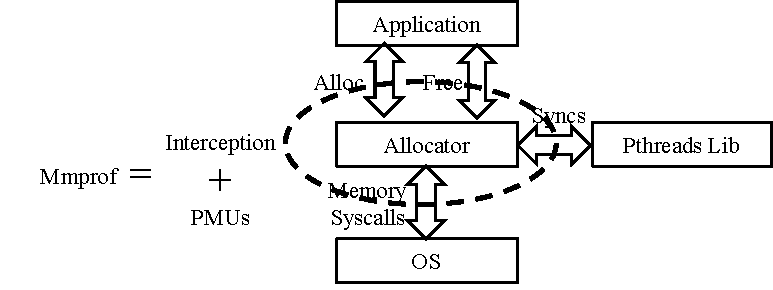
\includegraphics[width=3in]{paper/figures/basicidea.pdf}
\caption{Basic idea of \texttt{mmprof}.\label{fig:basicidea}}
\end{figure}

\MP{} is designed as a drop-in library that can be simply linked to applications (and allocators) with the preloading mechanism, which does not require the change or the re-compilation of applications and allocators, as far as an allocator utilizes standard synchronizations and system calls.

\MP{} aims to report important metrics of an allocator, as shown in Table~\ref{table:metrics}. These metrics help answer whether an allocator introduce performance or memory issues or not. If so, \MP{} further presents some details that help diagnose the particular design/implementation issue inside.  
%Table~\ref{table:metrics} also provides collection techniques for specific metrics, which are further discussed in Section~\ref{sec:idea}. 

\begin{table}[h]
  \centering
    \footnotesize
 % \setlength{\tabcolsep}{1.0em}
\begin{tabular}{l | l }
\hline
Category & Important Metrics \\ \hline
\multirow{2}{*}{Performance} & {Alloc/Free cycle} \\ \cline{2-2}
& {Cache misses, page faults, instructions} \\\hline
\multirow{3}{*}{Memory} & Internal fragmentation  \\ \cline{2-2}
	& Memory blowup  \\ \cline{2-2}
& {External fragmentation and others}  \\ \hline
\multirow{2}{*}{Scalability} & \specialcell{User space contention} \\ \cline{2-2}
& {Kernel space contention} \\ \hline
\multirow{3}{*}{\specialcell{Application \\ Friendliness}} & Cache/page utilization rate  \\ \cline{2-2}
& Passive/active false sharing \\ \cline{2-2}
& Cache invalidation rate \\ \hline
  \end{tabular}
 \caption{Important metrics of evaluating an allocator.\label{table:metrics}}
\end{table}

Since all allocators provide the same APIs to applications, invoke a limited set of system calls, and employ the similar thread synchronization primitives, \MP{} intercepts the interactions between an allocator and other components of the system, such as the application (memory allocations and deallocations), the OS (memory-related system calls), and the pthreads library (synchronization APIs). The basic idea of \MP{} is shown as Fig.~\ref{fig:basicidea}. Basically, it intercepts function invocations between the allocator and other components in the system.
%, and utilizes PMUs to collect memory accesses inside and outside each memory management operation, in order to help diagnose the performance issue. 
 
In order to collect the runtime of each interaction, \MP{} further employs the Time-Stamp Counter with the RDTSC instruction~\cite{coorporation1997using}. The Time-Stamp Counter is a hardware register available in X86 computers, which tracks the number of cycles since the reset time. The RDTSC instruction has two advantages over a system call to get the time, such as \texttt{gettimeofday}. First, its overhead is much lower than invoking a system call, typically around 30~60  cycles~\cite{rdtscoverhead}, instead of thousands of cycles. Second, it provides a fine-grained information (e.g., cycles), instead of microseconds that a system call can provide~\cite{pitfallsrdtsc}. With the RDTSC instruction, \MP{} obtains the timestamp before and after each operation, and uses the difference of timestamps as the runtime of a specific operation. \MP{} is able to measure the averaged runtime of each system call, each synchronization, and each memory management operation. Further, \MP{} also tracks user space contention by checking the status of locks, and infers kernel contention by the runtime of system calls. 

However, the information is still not efficient to explain some design issues inside and an allocator's application friendliness. \MP{} further employs hardware Performance Monitoring Units (PMU) to collect the information of memory accesses and hardware events. As shown in Fig.~\ref{fig:basicidea}, \MP{} focuses on accesses and events for both inside and outside of each memory management operation. The PMU hardware is ubiquitous in modern architectures~\cite{AMDIBS:07, IntelArch:PEBS:Sept09, armpmu}, and has been  employed to sample memory accesses or hardware-related events~\cite{DBLP:conf/sc/ItzkowitzWAK03, ibs-sc, Sheng:2011:RLN:1985793.1985848}.
%, such as memory loads and stores, hardware instructions, cache misses, and TLB misses
%For each sampled memory access, PMUs provides the type of an access (load or store), and instruction position, timestamp, and memory address. 
\MP{} utilizes sampled memory accesses to identify cache invalidation rate, false sharing effect, cache utilization rate, and page utilize rate, as discussed in Section~\ref{sec:profilefriendliness}. \MP{} employs PMUs to collect the number of instructions, page faults, and cache misses for each memory management operation. Therefore, \MP{} helps programmers identify particular design issues inside an allocator. 

%Overall, \MP{} reports all metrics listed in Table~\ref{table:metrics}, by employing  RDTSC and PMUs techniques. The reported data, when combined together, explains the performance, scalability, memory consumption of an allocator. 
%The reported data will benefit both allocator designers and normal programmers. 
%I helps predict the potential performance issue of an allocator. 

\begin{comment}

\subsection{Technical Challenges}

As described above, \MP{} employs hardware PMUs, time-stamp counters, and simple counters together to perform the profiling. But there exist some technical challenges as follows. 

The first important challenge is the overhead challenge, where a careless design may impose up to 100 $\times$ overhead based on our development experience. The huge overhead could be unaffordable even for development phases. More importantly, the significant overhead may also skew the evaluation results unnecessarily. Therefore, \MP{} balances the overhead and the precision of data collection (Section~\ref{sec:profilingmemory}), and designs some efficient mechanisms to perform the collection, such as three-level lookup mechanism of Section~\ref{sec:profilefriendliness}. 

The second challenge is to evaluate some metrics that were proposed a long time ago, but without no practical evaluation, such as memory blowup~\cite{Hoard}, passive/active false sharing~\cite{Hoard}. The reason is possibly due to no existing allocator profilers. Therefore, people tends to design  synthetic benchmarks to evaluate the performance of an allocator~\cite{Hoard, Scalloc}, without presenting quantitative evaluation. 

%The third challenge is to balance the efficiency, interference, and correctness. 

%Statistically. 

The third challenge is to deal with thread migration caused by the underlying OS scheduler. Based on our understanding, every core has its own registers for timestamps and hardware events. Therefore, when a thread is scheduled to a different core, the reported value that subtracts the data of the new core to that of the old one might be incorrect. One solution is to bind every thread to a different core. However, it may  skew the profiling results, caused by the binding. Instead, \MP{} takes no action by assuming that the thread migration is a rare event. Therefore, some migrations should not change the accuracy of the averaged data. 

%Therefore, a naive design without controlling thread binding may actually skew the evaluation results. For instance, during our development,  

The last challenge is to predict the performance impact of an allocator. The reported metrics could benefit allocator designers/programmers by providing the details of each operation, each lock, each system call, and cache friendliness. The reported data may also benefit normal users by providing the detailed memory overhead. However, it is not very clear whether a better allocator is required or not, in terms of the performance. Therefore, \MP{} tries to predict the potential performance improvement if using an efficient allocator so that the report can also benefit an un-experienced programmer or normal user. However, it is very challenge to do this, since the performance can be affected by multiple factors, such as the parallelization and the frequency of allocations.    

 

%Except the above challenges, there are other small challenges come from the adaption to different allocators. Specific issues include the following ones: (1) How to obtain the specific details of different allocators, such as size class information, type of allocator, metadata size information? (Section~\ref{sec:understandingallocators}) (2) How to design a general but fast lookup mechanism for different allocators? (3) How to profile kernel-contention for allocators?



% Comparing to the method of utilizing system calls, such as \texttt{gettimeofday()}, the RDTSC instruction has two advantages. First, the overhead is much lower than issuing a system call, typically around 25-35 cycles~\cite{rdtscoverhead}. Second, it provides a high-resolution timer, with the granularity of cycles, which is much finer than traditional system calls~\cite{pitfallsrdtsc}. For instance, the system call \texttt{gettimeofday} could only provide the microsecond granularity, which is too coarse for measuring the performance of system calls or synchronization overhead.  


	
\end{comment}



